\documentclass{article}
\usepackage[a4paper, margin=2cm]{geometry}

% Math packages
\usepackage{amsthm, commath, bm}

% Physics stuff
\usepackage{physics}

% Graphics
\usepackage{tikz}
\usetikzlibrary{calc, arrows.meta}

% For code samples
\usepackage{listings}

%
\usepackage{booktabs}
\usepackage{hyperref}
% \usepackage{cleveref}

% Content related-stuff
\title{Some Course on Something}
\author{Peleg Bar Sapir}

%%%% MAIN DOC %%%%

\begin{document}
\maketitle

% For tests
\ifdefined\testcode
  \section{Tests}
  This is a test. And this is a reference to some code: \autoref{lst:code1}.
  \begin{lstlisting}[
	% there are many more options of styling, see the official documentation, these are just the defaults I like
	frame=single, % make single-line frame around the verbatim
	framesep=2mm, % put some more spacing between the frame and text
	aboveskip=5mm, % put some more space above the box
	basicstyle={\linespread{0.9}\small\ttfamily}, % use typewriter (monospace) font
	caption={I am some code.}, % set the caption text
	captionpos=b, % put the caption at the bottom (b) or top (t) or both (bt)
	label={lst:code1}, % label to be referenced via \ref{}
	numbers=left, % line numbers on the left
	numberstyle={\scriptsize\ttfamily\color{black!60}}, % the style for line numbers
	escapeinside={<@}{@>} % between those sequences are command evaluated
]
<@\textcolor[HTML]{3010CF}{\textit{\textbf{\texttt{import}}}}@><@\textcolor[HTML]{000000}{\texttt{\ }}@><@\textcolor[HTML]{000000}{\texttt{numpy}}@><@\textcolor[HTML]{000000}{\texttt{\ }}@><@\textcolor[HTML]{3010CF}{\textit{\textbf{\texttt{as}}}}@><@\textcolor[HTML]{000000}{\texttt{\ }}@><@\textcolor[HTML]{000000}{\texttt{np}}@>
<@\textcolor[HTML]{3010CF}{\textit{\textbf{\texttt{import}}}}@><@\textcolor[HTML]{000000}{\texttt{\ }}@><@\textcolor[HTML]{000000}{\texttt{numpy}}@><@\textcolor[HTML]{000000}{\texttt{.}}@><@\textcolor[HTML]{000000}{\texttt{typing}}@><@\textcolor[HTML]{000000}{\texttt{\ }}@><@\textcolor[HTML]{3010CF}{\textit{\textbf{\texttt{as}}}}@><@\textcolor[HTML]{000000}{\texttt{\ }}@><@\textcolor[HTML]{000000}{\texttt{npt}}@>


<@\textcolor[HTML]{777777}{\textit{\texttt{\#\ Axes}}}@>
<@\textcolor[HTML]{EA5110}{\texttt{X\_}}@><@\textcolor[HTML]{000000}{\texttt{,\ }}@><@\textcolor[HTML]{EA5110}{\texttt{Y\_}}@><@\textcolor[HTML]{000000}{\texttt{,\ }}@><@\textcolor[HTML]{EA5110}{\texttt{Z\_}}@><@\textcolor[HTML]{000000}{\texttt{\ }}@><@\textcolor[HTML]{1041FF}{\texttt{=}}@><@\textcolor[HTML]{000000}{\texttt{\ }}@><@\textcolor[HTML]{000000}{\texttt{np}}@><@\textcolor[HTML]{000000}{\texttt{.}}@><@\textcolor[HTML]{2387FF}{\texttt{ones}}@><@\textcolor[HTML]{000000}{\texttt{(}}@><@\textcolor[HTML]{DE6F10}{\texttt{3}}@><@\textcolor[HTML]{000000}{\texttt{)}}@>
<@\textcolor[HTML]{000000}{\texttt{}}@>
<@\textcolor[HTML]{777777}{\textit{\texttt{\#\ NumPy\ types}}}@>
<@\textcolor[HTML]{724BFF}{\textit{\texttt{NDArrayFloat}}}@><@\textcolor[HTML]{000000}{\texttt{\ }}@><@\textcolor[HTML]{1041FF}{\texttt{=}}@><@\textcolor[HTML]{000000}{\texttt{\ }}@><@\textcolor[HTML]{000000}{\texttt{npt}}@><@\textcolor[HTML]{000000}{\texttt{.}}@><@\textcolor[HTML]{2387FF}{\texttt{NDArray}}@><@\textcolor[HTML]{000000}{\texttt{[}}@><@\textcolor[HTML]{000000}{\texttt{np}}@><@\textcolor[HTML]{000000}{\texttt{.}}@><@\textcolor[HTML]{2387FF}{\texttt{float\_}}@><@\textcolor[HTML]{000000}{\texttt{]}}@>
<@\textcolor[HTML]{000000}{\texttt{}}@>

<@\textcolor[HTML]{777777}{\textit{\texttt{\#\ Functions}}}@>
<@\textcolor[HTML]{3010CF}{\textit{\textbf{\texttt{def}}}}@><@\textcolor[HTML]{000000}{\texttt{\ }}@><@\textcolor[HTML]{255CFF}{\texttt{normalize}}@><@\textcolor[HTML]{000000}{\texttt{(}}@><@\textcolor[HTML]{000000}{\texttt{vec}}@><@\textcolor[HTML]{000000}{\texttt{:\ }}@><@\textcolor[HTML]{1F8F42}{\texttt{NDArrayFloat}}@><@\textcolor[HTML]{000000}{\texttt{)\ }}@><@\textcolor[HTML]{1041FF}{\texttt{->}}@><@\textcolor[HTML]{000000}{\texttt{\ }}@><@\textcolor[HTML]{1F8F42}{\texttt{NDArrayFloat}}@><@\textcolor[HTML]{000000}{\texttt{:}}@>
<@\textcolor[HTML]{000000}{\texttt{}}@><@\textcolor[HTML]{000000}{\texttt{\ \ \ \ }}@><@\textcolor[HTML]{EA5110}{\texttt{L}}@><@\textcolor[HTML]{000000}{\texttt{:\ }}@><@\textcolor[HTML]{1F8F42}{\texttt{float}}@><@\textcolor[HTML]{000000}{\texttt{\ }}@><@\textcolor[HTML]{1041FF}{\texttt{=}}@><@\textcolor[HTML]{000000}{\texttt{\ }}@><@\textcolor[HTML]{000000}{\texttt{np}}@><@\textcolor[HTML]{000000}{\texttt{.}}@><@\textcolor[HTML]{2387FF}{\texttt{linalg}}@><@\textcolor[HTML]{000000}{\texttt{.}}@><@\textcolor[HTML]{2387FF}{\texttt{norm}}@><@\textcolor[HTML]{000000}{\texttt{(}}@><@\textcolor[HTML]{000000}{\texttt{vec}}@><@\textcolor[HTML]{000000}{\texttt{)}}@>
<@\textcolor[HTML]{000000}{\texttt{}}@><@\textcolor[HTML]{000000}{\texttt{\ \ \ \ }}@><@\textcolor[HTML]{3010CF}{\textit{\textbf{\texttt{assert}}}}@><@\textcolor[HTML]{000000}{\texttt{\ }}@><@\textcolor[HTML]{EA5110}{\texttt{L}}@><@\textcolor[HTML]{000000}{\texttt{\ }}@><@\textcolor[HTML]{1041FF}{\texttt{!=}}@><@\textcolor[HTML]{000000}{\texttt{\ }}@><@\textcolor[HTML]{DE6F10}{\texttt{0.}}@><@\textcolor[HTML]{000000}{\texttt{,\ }}@><@\textcolor[HTML]{418310}{\texttt{"Can't\ normalize\ the\ zero\ vector."}}@>
<@\textcolor[HTML]{000000}{\texttt{\ \ \ \ }}@><@\textcolor[HTML]{3010CF}{\textit{\textbf{\texttt{return}}}}@><@\textcolor[HTML]{000000}{\texttt{\ }}@><@\textcolor[HTML]{000000}{\texttt{vec}}@><@\textcolor[HTML]{000000}{\texttt{\ }}@><@\textcolor[HTML]{1041FF}{\texttt{/}}@><@\textcolor[HTML]{000000}{\texttt{\ }}@><@\textcolor[HTML]{EA5110}{\texttt{L}}@>


<@\textcolor[HTML]{3010CF}{\textit{\textbf{\texttt{def}}}}@><@\textcolor[HTML]{000000}{\texttt{\ }}@><@\textcolor[HTML]{255CFF}{\texttt{scale}}@><@\textcolor[HTML]{000000}{\texttt{(}}@><@\textcolor[HTML]{000000}{\texttt{vec}}@><@\textcolor[HTML]{000000}{\texttt{:\ }}@><@\textcolor[HTML]{1F8F42}{\texttt{NDArrayFloat}}@><@\textcolor[HTML]{000000}{\texttt{,\ }}@><@\textcolor[HTML]{000000}{\texttt{a}}@><@\textcolor[HTML]{000000}{\texttt{:\ }}@><@\textcolor[HTML]{1F8F42}{\texttt{float}}@><@\textcolor[HTML]{000000}{\texttt{)\ }}@><@\textcolor[HTML]{1041FF}{\texttt{->}}@><@\textcolor[HTML]{000000}{\texttt{\ }}@><@\textcolor[HTML]{1F8F42}{\texttt{NDArrayFloat}}@><@\textcolor[HTML]{000000}{\texttt{:}}@>
<@\textcolor[HTML]{000000}{\texttt{}}@><@\textcolor[HTML]{000000}{\texttt{\ \ \ \ }}@><@\textcolor[HTML]{3010CF}{\textit{\textbf{\texttt{return}}}}@><@\textcolor[HTML]{000000}{\texttt{\ }}@><@\textcolor[HTML]{255CFF}{\texttt{normalize}}@><@\textcolor[HTML]{000000}{\texttt{(}}@><@\textcolor[HTML]{000000}{\texttt{vec}}@><@\textcolor[HTML]{000000}{\texttt{)\ }}@><@\textcolor[HTML]{1041FF}{\texttt{*}}@><@\textcolor[HTML]{000000}{\texttt{\ }}@><@\textcolor[HTML]{000000}{\texttt{a}}@>

\end{lstlisting}


  And this is a TikZ drawing: \autoref{fig:tikztest}.

  \begin{figure}
      \begin{center}
      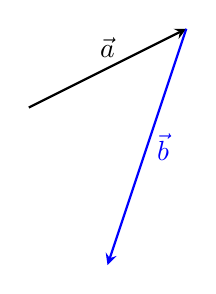
\begin{tikzpicture}
        \draw[-stealth, thick] (0,0) -- (2,1) node[midway, above] {$\vec{a}$};
        \draw[-stealth, thick, blue] (2,1) -- ++(-1,-3) node[midway, right] {$\vec{b}$};
      \end{tikzpicture}
      \end{center}
    \caption{A figure.}\label{fig:tikztest}
  \end{figure}
  
\else
\fi

% Content
\section{Introduction}
\subsection{Why are Simulations Used?}
\subsection{Python}
\subsection{A Bit About Git}
\subsection{Some Mathematical Background}

\section{Simulating Simple Mechanics}
\subsection{Forward Euler Method}
\subsection{Backward Euler Method}
\subsection{Verlet Integration}
\subsection{Runge-Kutta Method}

\section{Thermodynamics}

\section{Waves}

\section{Molecular Dynamics}


\end{document}
